%-----------------------------------------------------------------------------------------------------
%	INCLUSIÓN DE PAQUETES BÁSICOS
%-----------------------------------------------------------------------------------------------------
\documentclass{article}
%--------------------------------------------------------------------------------------------------
%	SELECCIÓN DEL LENGUAJE
%--------------------------------------------------------------------------------------------------

\usepackage[utf8]{inputenc}                           \usepackage{changepage} % adjust table

%--------------------------------------------------------------------------------------------------
%	SELECCIÓN DE LA FUENTE
%--------------------------------------------------------------------------------------------------
% Fuente utilizada.
\usepackage{courier}                    % Fuente Courier.
\usepackage{microtype}                  
%--------------------------------------------------------------------------------------------------
%	ALGORITMOS
%--------------------------------------------------------------------------------------------------
\usepackage{algpseudocode}
\usepackage{algpseudocode}
\usepackage{algorithm}
\renewcommand{\thealgorithm}{}
%--------------------------------------------------------------------------------------------------
%	IMÁGENES
%--------------------------------------------------------------------------------------------------
\usepackage{float}
\usepackage{placeins}
%--------------------------------------------------------------------------------------------------
%	ESTILO DE PÁGINA
%--------------------------------------------------------------------------------------------------
% Paquetes para el diseño de página:
\usepackage{fancyhdr}              
\usepackage{lastpage}              
\usepackage{extramarks}             
\usepackage[parfill]{parskip}      
\usepackage{geometry}               
\pagestyle{fancy}
\geometry{left=3cm,right=3cm,top=3cm,bottom=3cm,headheight=1cm,headsep=0.5cm} 
\fancyhf{}
\linespread{1.1}                        % Espacio entre líneas.
\setlength\parindent{0pt}               % Selecciona la indentación para cada inicio de párrafo.
\renewcommand\headrule{
	\begin{minipage}{1\textwidth}
	    \hrule width \hsize
	\end{minipage}
}
% Texto de la cabecera:
\lhead{\subject}                          % Parte izquierda.
\chead{}                                    % Centro.
\rhead{\doctitle \ - \docsubtitle}              % Parte derecha.
% Pie de página del documento. Se ajusta la línea del pie de página.
\renewcommand\footrule{
\begin{minipage}{1\textwidth}
    \hrule width \hsize
\end{minipage}\par
}
\lfoot{}                                                 % Parte izquierda.
\cfoot{}                                                 % Centro.
\rfoot{Page\ \thepage\ de\ \protect\pageref{LastPage}} % Parte derecha.


%----------------------------------------------------------------------------------------
%   MATEMÁTICAS
%----------------------------------------------------------------------------------------

% Paquetes para matemáticas:
\usepackage{amsmath, amsthm, amssymb, amsfonts, amscd}
\usepackage{proof}
 % Teoremas, fuentes y símbolos.
\usepackage{tikz-cd} % para diagramas conmutativos
\usepackage[mathscr]{euscript}
\let\euscr\mathscr \let\mathscr\relax% just so we can load this and rsfs
\usepackage[scr]{rsfso}
\newcommand{\powerset}{\raisebox{.15\baselineskip}{\Large\ensuremath{\wp}}}
 % Nuevo estilo para definiciones
 \newtheoremstyle{definition-style}
 {5pt}               
 {0pt}                
 {}                  
 {}                   
 {\bf}             
 {.}                 
 {\newline}               
 {}                 

 % Nuevo estilo para teoremas
 \newtheoremstyle{theorem-style} % Nombre del estilo
 {5pt}                % Espacio por encima
 {0pt}                % Espacio por debajo
 {\itshape}           % Fuente del cuerpo
 {}                   % Identación: vacío= sin identación, \parindent = identación del parráfo
 {\bf}                % Fuente para la cabecera
 {.}                  % Puntuación tras la cabecera
 {\newline}               % Espacio tras la cabecera: { } = espacio usal entre palabras, \newline = nueva línea
 {}                   % Especificación de la cabecera (si se deja vaía implica 'normal')

 % Nuevo estilo para ejemplos y ejercicios
 \newtheoremstyle{example-style} % Nombre del estilo
 {5pt}                % Espacio por encima
 {0pt}                % Espacio por debajo
 {}                   % Fuente del cuerpo
 {}                   % Identación: vacío= sin identación, \parindent = identación del parráfo
 {\scshape}                % Fuente para la cabecera
 {:}                  % Puntuación tras la cabecera
 {.5em}               % Espacio tras la cabecera: { } = espacio usal entre palabras, \newline = nueva línea
 {}                   % Especificación de la cabecera (si se deja vaía implica 'normal')

 % Teoremas:
 \theoremstyle{theorem-style}  
 \newtheorem{theorem}{Theorem}[section]  
 \newtheorem{corollary}[theorem]{Corollary} 
 \newtheorem{lemma}[theorem]{Lemma}
 \newtheorem{proposition}[theorem]{Proposition}

 % Definiciones, notas, conjeturas
 \theoremstyle{definition-style}
 \newtheorem{definition}{Definition}[section]
 \newtheorem{conjecture}{Conjecture}[section]
 \newtheorem*{note}{Note} 

 % Ejemplos, ejercicios
 \theoremstyle{example-style}
 \newtheorem{example}{Example}[section]
 \newtheorem{exercise}{Ejercicio}[section]
 
 % Listas ordenadas con números romanos (i), (ii), etc.
\newenvironment{nlist}
{\begin{enumerate}
\renewcommand\labelenumi{(\emph{\roman{enumi})}}}
{\end{enumerate}}
%commutative-diagrams
\usepackage{tikz-cd}
% code listings 
\usepackage{listings}

%-----------------------------------------------------------------------------------------------------
%	BIBLIOGRAFÍA
%-----------------------------------------------------------------------------------------------------

\usepackage[backend=bibtex, style=numeric, sorting = none]{biblatex}
\usepackage{csquotes}

\addbibresource{references.bib}

%-----------------------------------------------------------------------------------------------------
%	PORTADA
%-----------------------------------------------------------------------------------------------------
% Elija uno de los siguientes formatos.
% No olvide incluir los archivos .sty asociados en el directorio del documento.
\usepackage{title1}
%\usepackage{title2}
%\usepackage{title3}

%-----------------------------------------------------------------------------------------------------
%	TÍTULO, AUTOR Y OTROS DATOS DEL DOCUMENTO
%-----------------------------------------------------------------------------------------------------

% Título del documento.
\newcommand{\doctitle}{Some ideas for the introduction of reasoning techniques in Welder}
% Subtítulo.
\newcommand{\docsubtitle}{July-August 2017}
% Fecha.
\newcommand{\docdate}{}
% Asignatura.
\newcommand{\subject}{}
% Autor.
\newcommand{\docauthor}{Rodrigo Raya Castellano}
\newcommand{\docaddress}{}
\newcommand{\docemail}{}

%-----------------------------------------------------------------------------------------------------
%	RESUMEN
%-----------------------------------------------------------------------------------------------------

% Resumen del documento. Va en la portada.
% Puedes también dejarlo vacío, en cuyo caso no aparece en la portada.
%\newcommand{\docabstract}{}
\newcommand{\docabstract}{}

\begin{document}

\maketitle

%-----------------------------------------------------------------------------------------------------
%	ÍNDICE
%-----------------------------------------------------------------------------------------------------

% Profundidad del Índice:
%\setcounter{tocdepth}{1}

\newpage
\tableofcontents
\newpage

\section{Contributions to Welder}
\subsection{Setup to use Welder in Intellij Idea}

One of the main difficulties to prove theorems in Welder when we first approached the assistant was the fact that errors where really difficult to deal with. Errors could come not only from Welder, but from Inox (we actually uncover some bugs in the least used parts of the system) or just because what we wanted to prove was not true. 

We believe that having a proper way to debug proofs could not only reduce the learning curve of new users but also facilitate that new users acquire a better understanding of the SMT solver $\to$ Inox $\to$ Welder stack. The following explains a possible setup for Welder to run on Intellij Idea IDE. 

On Intellij Idea 2017.2.1 we create a new Scala SBT-based project. In the file build.sbt we write the following:

\begin{figure}[H]
\centering
\makebox[\textwidth][c]{
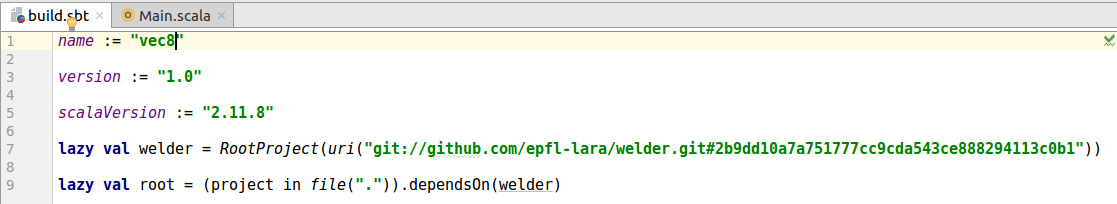
\includegraphics[scale=0.4]{./images/capt4.png}
}
\end{figure}

Next, we go to File $\to$ Settings $\to$ Build,Execution,Deployment $\to$ Build Tools $\to$ SBT and mark the option \textit{Use SBT shell for build and import (requires sbt 0.13.5+)} and press OK.

\begin{figure}[H]
\centering
\makebox[\textwidth][c]{
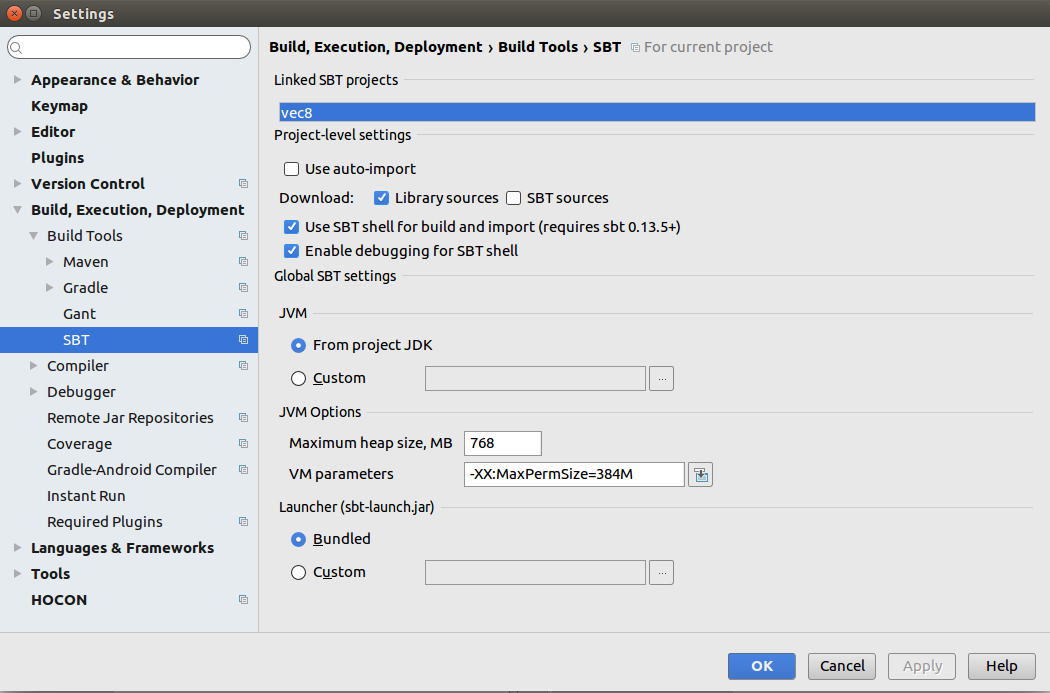
\includegraphics[scale=0.3]{./images/capt1.png}
}
\end{figure}

Finally, we select the option Refresh project that should have appeared after updating the build.sbt file. We accept, without unmarking the removal of the modules that Intellij Idea suggests. 

Once we are done, we obtain in the Project Panel three projects modules. Observe that the RootProject command in the build.sbt is highlighted. We can get rid of this by renaming the projects and build files to the following:

\begin{enumerate}
\item inox-root and inox-root-build
\item myproject-root and myproject-root-build
\item welder-root and welder-root-build
\end{enumerate}

To do so right click and the modules and then Refactor $\to$ Rename $\to$ Rename Module. Before building our project, we mark the src file in our project as source file in File $\to$ Project-Structure $\to$ Project name $\to$ Sources $\to$ src and selecting Sources icon. Then we put our Main.scala file in the corresponding directory. 

\begin{figure}[H]
\centering
\makebox[\textwidth][c]{
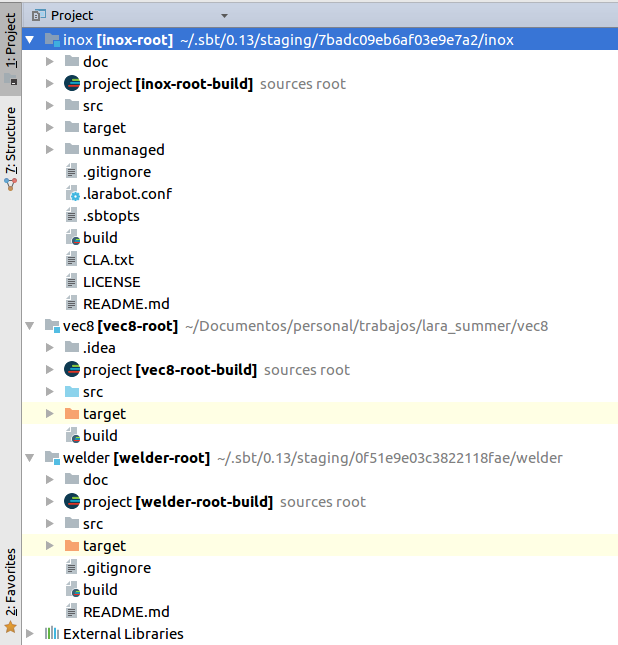
\includegraphics[scale=0.3]{./images/capt2.png}
}
\end{figure}

We also need to tell Intellij Idea that our project depends on Inox. We do so in File $\to$ Project-Structure $\to$ Project name $\to$ + $\to$ Module dependency... $\to$ inox-root.

\begin{figure}[H]
\centering
\makebox[\textwidth][c]{
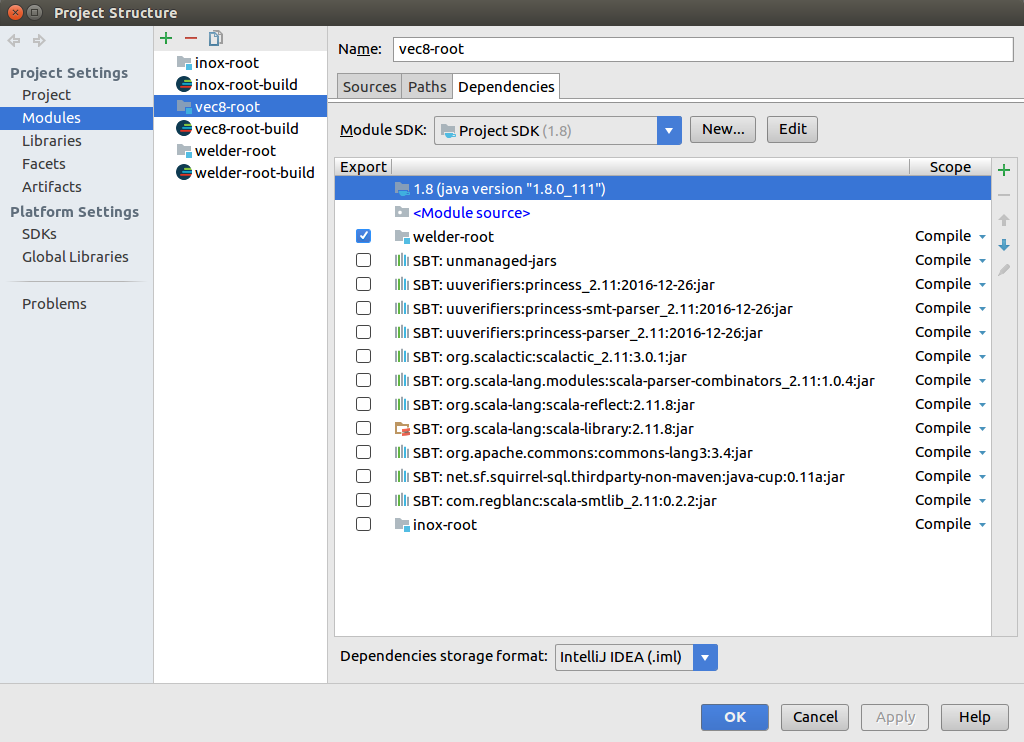
\includegraphics[scale=0.3]{./images/capt3.png}
}
\end{figure}

We set the running configuration in Run $\to$ Edit configuration $\to$ Application mode and selecting the module and the main program as usual. Before running this, we go to the SBT shell and compile the program. Finally, we run the Application as usual in Intellij Idea. 

The above configuration process can be found in references \cite{ref1}-\cite{ref7}.
\subsection{Adding the first "naive" tactics}

During the course, we learnt that much of the effort in proving theorems happens while finding the appropiate inductive hypothesis. In fact, many direct goals are not solved by the underlying SMT solver. 

On the other hand, most of the literature that we are aware of works at low level on the SMT solver such as in \cite{leino} or \cite{kuncak}. We carried out experiments to use some of the strategies described in these papers but the results did not change. 

Therefore, we concluded that in order to provide a first example of tactic in Welder it should be as simple as a method that allows the user to perform automatic induction by providing automatically the inductive hypothesis on the sub-trees of the algebraic data types. 

Here is an example of how this new syntax would look 
like:

\begin{lstlisting}[caption=Proposed induct syntax,captionpos = b]
lazy val lemma: Theorem = {
 def property(l: Expr) = {
  forall("i" :: IntegerType, "j" :: IntegerType){ case (i,j) =>
   (i >= 0 && j >= 0) ==> (drop(l,i+j) === drop(drop(l,j),i))
  }
 }
 induct(property _, "l" :: T(list))
}
\end{lstlisting} 

The above example would succeed in proving $\forall l: List,i:Nat,j:Nat.drop(l,i+j) === drop(drop(l,j),i)$. In any case, we recommend to use the version of Welder used in the online reference of the project \cite{project} for testing the examples. 

Essentially the two summarized versions of the induction constructs we implemented are as follows:

\begin{lstlisting}[caption=Proposed induct signatures to be found in Tactics.scala,captionpos = b]
def induct(property: Expr => Expr, valDef: ValDef): Attempt[Theorem] 
def natInduct(property: Expr => Expr, base: Expr,
              baseCase: Goal => Attempt[Witness]): Attempt[Theorem] 
\end{lstlisting} 
  
which perform structural and natural induction respectively. 

It was not easy to find other easy examples of implementable tactics which motivates the second part of our work in which we tried to investigate Term Rewriting techniques in order to solve automatically theorems that we proved in the elliptic curves work carried out during the semester. 







\newpage
\section{Term rewriting}

\subsection{Motivation}

After the practical work that we carried out to improve the way in which the developer relates with Welder, it turned out that more interesting strategies were necessary to turn Welder into a real proof assistant. We found a possible solution in \cite{term-rewriting} and used \cite{handbook} as further support.

As a motivating example, we consider the problem of determining if a given equation holds in group theory. This is not far from our elliptic curve project, since in several occasions we had to manually deduce easy properties of fields that only require basic reasoning.  Given the axioms that define a group: \begin{alignat*}{5}
(G1) \; & (xy)z \; & \approx & \; x(yz) \\
(G2) \; & ex  \; & \approx & \;  x \\
(G3) \; & x^{-1}x \; & \approx & \; e 
\end{alignat*} where as usual $e$ denotes the neutral element of the group and $x^{-1}$ denotes the inverse. We can for instance try to decide if equation $e = xx^{-1}$ holds. This is the so-called word problem:

\begin{definition}[The word problem informally]
Given a set of identities $E$ and two terms $s,t$, determine if it is possible to derive $t$ from $s$ using $E$ as a set of rewriting equations in both directions. 
\end{definition}

Using $E = \{G_1,G_2,G_3\}$ we can derive term $t = xx^{-1}$ from term $s = e$: $$e \stackrel{G3}{\approx} (xx^{-1})^{-1}(xx^{-1}) \stackrel{G2}{\approx} (xx^{-1})^{-1}(x(ex^{-1})) \stackrel{G3}{\approx} (xx^{-1})^{-1}(x((x^{-1}x)x^{-1}))
\stackrel{G1}{\approx} (xx^{-1})^{-1}((x(x^{-1}x))x^{-1})
$$ $$
\stackrel{G1}{\approx} (xx^{-1})^{-1}(((xx^{-1})x)x^{-1})
\stackrel{G1}{\approx} (xx^{-1})^{-1}((xx^{-1})(xx^{-1}))
\stackrel{G1}{\approx} ((xx^{-1})^{-1}(xx^{-1}))(xx^{-1})
\stackrel{G3}{\approx} e(xx^{-1})
\stackrel{G2}{\approx} xx^{-1}
$$

It is clear that the amount of rewriting operations is unacceptable. Term rewriting proposes another strategy. One considers the identities in $E$ as uni-directional rewrite rules: \begin{alignat*}{5}
(RG1) \; & (xy)z \; & \to & \; x(yz) \\
(RG2) \; & ex  \; & \to & \;  x \\
(RG3) \; & x^{-1}x \; & \to & \; e 
\end{alignat*} Here the idea is that identities will be only be applied in the direction that simplifies a given term. The strategy is to look for terms such that no more rules apply, so-called normal forms. Given two terms $s,t$ we could:

\begin{enumerate}
\item Reduce them to normal forms $\hat s, \hat t$.
\item Check whether $\hat s, \hat t$ are syntactically equal.
\end{enumerate}

There are two problems with this approach:

\begin{enumerate}
\item Equivalent terms can have distinct normal forms. For instance, $xx^{-1}$ and $e$ are normal forms with respect to (RG1) and (RG2) and we have shown they are equivalent. The above method would fail because they are syntactically distinct. The property needed to have uniqueness of normal forms is called confluence. 

\item Normal forms may not exist. the process of reducing a term can lead to an infinite chain of rule applications. The property that ensures the existence of normal forms is called termination. 

If the rewrite system is not confluent we can use a technique called completion to extend it to a confluent one. In the case of groups, there exists a confluent and terminating extension.
\end{enumerate}
\subsection{Abstract reduction systems}

\begin{definition}[Abstract reduction system]
Given a set $A$ and a binary relation $\to$ in $A$.

An abstract reduction system is a pair $(A,\to)$. The binary relation $\to$ can be seen to represent computation steps. 

We note $(a,b) \in \to$ as $a \to b$. 
\end{definition}

We want to determine if two terms are equivalent, that is, if $a \stackrel{*}{\leftrightarrow} b$. Our strategy is the one that we pointed out in the examples about groups: to reduce to a certain normal form that has a uniqueness property. The advantage of this approach is that an undirected search on $\to$ and $\gets$ would be too expensive. First we need some notation for operations that are based on the composition of relations: 

Given $R \subseteq A \times B \land S \subseteq B \times C$ two relations, its composition is: $$R \circ S = \{(x,z) \in A \times C: \exists y \in B. (x,y) \in R \land (y,z) \in S\}$$

\begin{table}[H]
\centering
\begin{adjustwidth}{-2cm}{}
\begin{tabular}{|| c | c | c | c ||}
\hline
\hline & $\stackrel{0}{\rightarrow} = \{(x,x):x \in A \}$ & & $\stackrel{i+1}{\rightarrow} = \stackrel{i}{\rightarrow} \circ \to$ \\
\hline Transitive closure & $\stackrel{+}{\rightarrow} = \cup_{i > 0} \stackrel{i}{\rightarrow}$ & Reflexive transitive closure & $\stackrel{*}{\rightarrow} = \stackrel{+}{\rightarrow} \cup \stackrel{0}{\rightarrow}$ \\
\hline  Reflexive closure & $\stackrel{=}{\rightarrow} = \to \cup \stackrel{0}{\rightarrow}$ & Inverse & $\stackrel{-1}{\rightarrow} = \{(y,x):x \to y\}$ and $\leftarrow= \stackrel{-1}{\rightarrow}$ \\
\hline  Symmetric closure & $\leftrightarrow = \to \cup \leftarrow$ & Transitive symmetric closure & $\stackrel{+}{\rightarrow} = (\leftrightarrow)^+$ \\
\hline Reflexive, transitive, symmetric closure &  $\stackrel{*}{\rightarrow} = (\leftrightarrow)^*$ & & \\
\hline
\end{tabular}
\end{adjustwidth}
\caption{Notation for operations on relations}
\label{table:notation1}
\end{table}

We give some terminology for abstract reduction systems:

\begin{table}[H]
\centering
\begin{tabular}{|| c | c | c | c ||}
\hline
\hline x is reducible & $\exists y. x \to y$ & 
x is irreducible or in normal form  & $!\exists y. x \to y$ \\
\hline y is a normal form of x & $x \stackrel{*}{\rightarrow} y \land y$ is in normal form & unique normal form of x (if exists) & $x\downarrow$ \\
\hline y is direct successor of x & $x \to y$ &
y is successor of x & $x \stackrel{+}{\rightarrow} y$ \\
\hline x and y are joinable & $\exists z \in x \stackrel{*}{\rightarrow} z \stackrel{*}{\leftarrow} y$ & x,y joinable & $x \downarrow y$ \\
\hline
\end{tabular}
\caption{Terminology for the elements of the reduction system}
\label{table:notation2}
\end{table}


And some terminology for reductions:

\begin{table}[H]
\centering
\begin{adjustwidth}{-2cm}{}
\begin{tabular}{|| c | c | c | c ||}
\hline
\hline Church-Rosser & $x \stackrel{*}{\leftrightarrow} y \implies x \downarrow y$ & Semi-confluent & $y_1 \leftarrow x \stackrel{*}{\rightarrow} y_2 \implies y_1 \downarrow y_2$ \\
\hline Confluent & $y_1 \stackrel{*}{\leftarrow} x \stackrel{*}{\rightarrow} y_2 \implies y_1 \downarrow y_2$ & Terminating & there is no infinite descending chain $a_0 \to a_1 \to \cdots$ \\
\hline Normalizing & every element has a normal form & Convergent & confluent and terminating \\
\hline
\end{tabular}
\end{adjustwidth}
\caption{Terminology for reductions in reductions systems}
\label{table:notation3}
\end{table}

\begin{figure}[H]
\centering
\begin{tikzcd}
x \arrow[rr, leftrightarrow, "*"] \arrow[dr, dashrightarrow, "*"'] 
 &  & y \arrow[dl, dashrightarrow, "*"] \\
 & z &
\end{tikzcd}
\begin{tikzcd}
x \arrow[r, "*"] \arrow[d, "*"'] 
&  y_1 \arrow[d, dashed, "*"] \\
y_2 \arrow[r, dashed, "*"] & z
\end{tikzcd}
\begin{tikzcd}
x \arrow[r] \arrow[d, "*"] 
&  y_1 \arrow[d, dashed, "*"] \\
y_2 \arrow[r, dashed, "*"] & z
\end{tikzcd}
\caption{Church-Rosser, confluence and semi-confluence diagrams}
\end{figure}

\begin{proposition}[Relation between the properties of an abstract reduction system] 
The following propositions relate the properties of abstract reduction systems:

\begin{enumerate}
\item Any terminating relation is normalizing. The converse is not true. 
\item Church-Rosser $\iff$ Confluence $\iff$ Semi-confluence. 
\item Given a confluent relation $\to$ and $x \stackrel{*}{\leftrightarrow} y$:

1. y is in normal form $ \implies x \stackrel{*}{\rightarrow} y$\\
2. x,y are in normal form $ \implies x = y$. 
\end{enumerate}
\end{proposition}
\begin{proof}
\begin{enumerate}
\item Clearly, every terminating relation arrives to a normal form from any initial term. For the converse, consider the following acyclic, confluent and non-terminating relation:

\begin{tikzcd}
\cdot \arrow[r] \arrow[d] 
&  \cdot \arrow[r] \arrow{dl} 
& \cdot \arrow{dll} \arrow{r}
& \cdot \arrow{dlll}
& \cdots \\
\cdot 
\end{tikzcd}

\item 1) $\implies$ 2). Assume $y_1 \stackrel{*}{\leftarrow} x \stackrel{*}{\rightarrow} y_2$ then $x \stackrel{*}{\leftrightarrow} y$ and by Church-Rosser $\exists y_1 \downarrow y_2$.

2) $\implies$ 3). Trivial.

3) $\implies$ 1). Assume $x \stackrel{*}{\leftrightarrow} y$. By induction, if $x = y$ then $x \downarrow y$. Assuming $x \stackrel{*}{\leftrightarrow} y \leftrightarrow y'$ and that $x \downarrow y$ we need to show $x \downarrow y'$. There are two cases:

\begin{tikzcd}
& & & y' \arrow{dl} \\
 x  \arrow[rr, leftrightarrow, "*"] \arrow[dr,dashed,"*"] & & y \arrow[dl,dashed,"*"] \\
& \cdot
\end{tikzcd} \hspace{3mm}
\begin{tikzcd}
x \arrow[rr,leftrightarrow,"*"] \arrow[dr,dashed,"*",swap] & & y \arrow[dr] \arrow[dl,dashed,"*"] \\
& z \arrow[dr,dashed,"*",swap] & & y' \arrow[dl,dashed,"*",swap] \\
& & \cdot
\end{tikzcd}

For the first case, we perform induction on the lower triangle and in the second, induction on the upper triangle and then semi-confluence for the quadrilateral.

\item We take advantage of the fact that confluence is equivalent to Church Rosser and consider the following diagrams:

\begin{tikzcd}
x \arrow[rr,leftrightarrow,"*"] \arrow[rr,bend right]  & & y 
\end{tikzcd} \hspace{3mm}
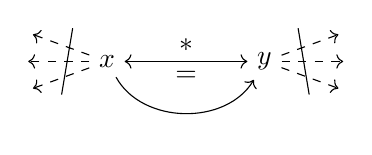
\begin{tikzpicture}

\node (x) at (0,0) {$x$};
\node (y) at (2,0) {$y$};

\draw[<->] (x) -- node[above] {$\ast$} node[below] {$=$} (y);
\draw[->] (x) to[bend right=60] (y);

\draw[->,dashed] (x) -- +(160:1);
\draw[->,dashed] (x) -- +(180:1);
\draw[->,dashed] (x) -- +(200:1);

\draw[->,dashed] (y) -- +(20:1);
\draw[->,dashed] (y) -- +(0:1);
\draw[->,dashed] (y) -- +(-20:1);

\draw ([yshift=12,xshift=-6]x.west) -- ([yshift=-12,xshift=-10]x.west);
\draw ([yshift=12,xshift=6]y.east) -- ([yshift=-12,xshift=10]y.east);

\end{tikzpicture}
\end{enumerate}
\end{proof}

\begin{proposition}[Results on the reduction strategy]
The following results give us hints on what conditions should we look for to apply the strategy of our motivation:

\begin{enumerate}
\item Condition for well-definition of $x\downarrow$:

\begin{enumerate}
\item $\to$ is confluent $\implies$ every element has at most one normal form.
\item $\to$ is normalizing and confluent $\implies$ every element has a unique normal form.
\end{enumerate}

\item Equivalence test with normal forms:

If $\to$ is confluent and normalizing then $x \stackrel{*}{\leftrightarrow} y \iff x\downarrow = y\downarrow$

\item Equivalence test with normal forms:

If $\to$ is convergent then $x \stackrel{*}{\leftrightarrow} y \iff x\downarrow = y\downarrow$
\end{enumerate}
\end{proposition}
\begin{proof}
\begin{enumerate}
\item 

\begin{enumerate}
\item If x has two normal forms $n_1^x,n_2^x$ by confluence we can join them. But since they're normal the only way to join them is that they are equal.
\item Use 1 to proof that the number of normal forms is $\le 1$ and normality to proof that it is $\ge 1$.
\end{enumerate}

\item $x \stackrel{*}{\leftrightarrow} y \implies x \downarrow \stackrel{*}{\leftrightarrow} y \implies x \downarrow \implies x \downarrow = y \downarrow$.

$x \downarrow = y \downarrow \implies x \stackrel{*}{\leftrightarrow} y$

\begin{tikzcd}
x \arrow[r,leftrightarrow,"*"] \arrow[d,leftrightarrow,"*",swap] & 
y \arrow[d,leftrightarrow,"*",swap] \\
x \downarrow \arrow[r,leftrightarrow,dashed,"*"] & y \downarrow
\end{tikzcd}

\item This a weaker result than the previous but note that in the search for normal forms, the previous one requires a breadth-first search which may be more costly in some situations. Therefore, literature focus on the convergent case. 
\end{enumerate}
\end{proof}


So now the question is, how do we prove confluence and termination?

\subsubsection{Termination}

Well-founded induction is a first tool to prove termination. It is a generalization of strong induction for natural numbers:

\begin{definition}[Strong induction for natural numbers]
Given property $P$ on natural numbers. 

$\forall n \in \mathbb{N}. P(n) \iff \forall n \in \mathbb{N}. (\forall m \in \mathbb{N}. m < n \implies P(m)) \implies P(n)$.
\end{definition}

Note that the base case for $0$ leaves the right hand-side with proving $P(0)$ just what we do in normal induction proofs. Now we abstract this principle from $(\mathbb{N},>)$ to any reduction system $(A,\to)$:

\begin{definition}[Well-founded induction (WFI) rule]
Given a property $P$ on the elements of $A$:\\

\infer{\forall x \in A. P(x)}{\forall x \in A. (\forall y \in A. x \stackrel{+}{\rightarrow} y \implies P(y)) \implies P(x)}
\end{definition}

In this case, the base case reduces to prove $P(x)$ for every $x$ without successor. It is interesting that this property holds exactly for terminating relations.

\begin{theorem}[Characterization of terminating relations]
Given $(A,\to)$ an abstract reduction system. 

WFI holds $\iff$ $\to$ terminates $\iff \forall B \subseteq A.\exists b \in B. \nexists b' \in B.b \to b'$
\end{theorem}
\begin{proof}
$\Rightarrow)$ Set $P(x) = $ there is no infinite chain starting from x. Given any $x$ the premise of WFI says that no successor of x has an infinite chain. Therefore, $x$ itself cannot have an infinite chain. Equivalently, $P(x)$ holds. 

$\Leftarrow)$ If WFI doesn't hold for $\to$ then there must exist $a_0 \in A$ such that: $$[\forall y \in A. a_0  \stackrel{+}{\rightarrow} y \implies P(y)) \implies P(a_0)] \land \lnot P(a_0)$$ Therefore there must exist $a_1 \in A$ such that: $$a_0 \stackrel{+}{\rightarrow} a_1 \land \lnot P(a_1)$$ This process repeats itself giving a chain: $$a_0 \stackrel{+}{\rightarrow} a_1 \stackrel{+}{\rightarrow} \cdots$$ that does not terminate.
\end{proof}

\begin{definition}[Properties related to termination]
A relation $\to$ is called:

\begin{enumerate}
\item \textbf{finitely branching} if each element has only a finite number of direct successors.
\item \textbf{globally finite} if each element has only finitely many successors.
\item \textbf{acyclic} if there is no element a such that $a \stackrel{+}{\rightarrow} a$. 
\end{enumerate}
\end{definition} 

\begin{proposition}[Relation between properties related to termination]
1. $\to$ terminating and finitely branching $\implies$ globally finite. \\
2. $\to$ acyclic and globally finite $\implies$ terminating. \\
3. $\to$ acyclic and finitely branching $\implies$ (globally finite $\iff$ terminating) \\
4. K\"onig's lemma: a finitely branching tree is infinite $\iff$ it contains an infinite path.
\end{proposition}

Different techniques to prove termination are presented in \cite{term-rewriting}. They imply the use of many orders such as lexicographic or multi-set orders which do not convey our main goal here of presenting general concepts towards completion algorithms. There is also an interesting comment on the characterization of termination with monotonic embeddings in $(\mathbb{N},>)$ for finitely branching relations.

\subsubsection{Confluence}

We now look at techniques to prove confluence. 

\begin{definition}[Other notions of confluence]
$\to$ is locally confluent $\iff \forall y_1,y_2 \in A. y_1 \gets x \to y_2 \implies y_1 \downarrow y_2$

$\to$ is strongly confluent $\iff \forall y_1,y_2,x.y_1 \gets x \to y_2 \implies \exists z.y_1 \stackrel{*}{\to} z \stackrel{=}{\gets} y_2$

$\to$ has the diamond property $\iff \forall y_1,y_2,x. y_1 \gets x \to y_2 \implies \exists z. y_1 \to z \gets y_2$
\end{definition}

Note that local confluence does not imply confluence as in the following example:

\begin{tikzcd} 
a  & 0 \arrow[r,bend left] \arrow[l] & 1 \arrow[r] \arrow[l,bend left] & b 
\end{tikzcd}

Note also that the diamond property is stronger than strong confluence. 

It is clear also that $\to$ is confluent $\iff$ $\stackrel{*}{\to}$ has the diamond property.

\begin{proposition}[Sufficient conditions for confluence]
The following are sufficient conditions to show confluence:

\begin{enumerate}
\item Newman's lemma: $\to$ terminating and locally confluent $\implies$ confluent.

\item $\to$ strongly confluent $\implies$ confluent.

\end{enumerate}
\end{proposition}
\begin{proof}
\begin{enumerate}
\item Well-founded induction on $P(x) = \forall y,z.y \stackrel{*}{\gets} x \stackrel{*}{\to} z \implies y \downarrow z$. We analyse $y \stackrel{*}{\gets} x \stackrel{*}{\to} z$:

\begin{enumerate}
\item If $x = y \lor x = z$ then $y \downarrow z$. 
\item In other case, $x \to y_1 \stackrel{*}{y} \land x \to z_1 \stackrel{*}{\to} z \stackrel{\text{local confluence}}{\implies} \exists u = y_1 \downarrow z_1$.

Since $x \stackrel{+}{\to} y_1 \land x \stackrel{+}{z_1} \stackrel{\text{ induction }}{\implies} \exists v = y \downarrow u \land w = v \downarrow z \implies \exists w = y_1 \downarrow z_1$
\end{enumerate}

\begin{tikzcd}
& & x \arrow[dl] \arrow[dr] & & \\
& y_1 \arrow[dl,"*",swap] \arrow[dr,dashed,"*"] & & z_1 \arrow[dl,dashed,"*",swap] \arrow[dr,"*"] & \\
y \arrow[dr,dashed,"*"] & & u \arrow[dl,dashed,"*",swap] & & z \arrow[ddll,dashed,"*",swap] \\
& v \arrow[dr,dashed,"*"] & & & \\
& & w & &
\end{tikzcd}

\item We prove semi-confluence with $y_1 \gets x_1 \stackrel{n}{\to} x_n \implies \exists y_n.y_1 \stackrel{*}{\to} y_n \stackrel{=}{\gets} x_n$ and we apply induction over $n$.

\begin{tikzcd} 
x_1 \arrow[r] \arrow[d] & x_2 \arrow[d,dashed,"="] & \ldots & x_{n-1} \arrow[d,dashed,"="] \arrow[r] & x_n \arrow[d,dashed,"="] \\
y_1 \arrow[r,dashed,"*"] & y_2  & \ldots & y_{n-1} \arrow[r,dashed,"="] & y_n
\end{tikzcd}
\end{enumerate}
\end{proof}

To use strong confluence property one defines given a relation $\to$, a stronly confluent relation $\to_s$ such that $\stackrel{*}{\to} = \stackrel{*}{\to_s}$ and by the theorem above we have that $\to$ is confluent ($\stackrel{*}{\to} = \stackrel{*}{\to_s} \implies \to_1 \text{ confluent } \iff \to_2 \text{ confluent }$). A sufficient condition for $\stackrel{*}{\to_1} = \stackrel{*}{\to_2}$ is $\to_1 \subseteq \to_2 \subseteq \stackrel{*}{\to_1}$. Therefore we have the following:

\begin{corollary}[Proving confluence by strong confluence]
If $\to_1 \subseteq \to_2 \subseteq \stackrel{*}{\to_1}$ and $\to_2$ is strongly confluent then $\to_1$ is confluent. 
\end{corollary}

Another strategy may be to split $\to = \to_1 \cup \to_2$ and prove that the confluence of each part gives the confluence of the total. The following concept is useful to prove this implication:

\begin{definition}[Commutation]
Two relations $\to_1,\to_2$:

\begin{enumerate}
\item commute: $\forall y_1,y_2,x.y_1 \stackrel{*}{\gets_1} x \stackrel{*}{\to_2} y_2 \implies \exists z.y_1 \stackrel{*}{\to_2} z \stackrel{*}{\gets_1} y_2 \iff \stackrel{*}{\gets_1} \circ \stackrel{*}{\to_2} \subseteq \stackrel{*}{\to_2} \circ \stackrel{*}{\gets_1}$
\item strongly conmute: $\forall y_1,y_2,x.y_1 \gets_1 x \to_2 y_2 \implies \exists z.y_1 \stackrel{=}{\to_2} z \stackrel{*}{\gets_1} y_2 \iff \gets_1 \circ \to_2 \subseteq \stackrel{=}{\to_2} \circ \stackrel{*}{\gets_1}$
\end{enumerate}
\end{definition}

\begin{proposition}[Commutation properties]
1. Commutation Lemma: If $\to_1,\to_2$ commute strongly then they commute.\\
2. Commutative Union Lemma: If $\to_1,\to_2$ are confluent and commute then $\to_1 \cup \to_2$ is confluent. 
\end{proposition}











\subsection{Universal algebra}

\subsubsection{General notions}

A way to formalize the notion of computation is to introduce multi-typed algebraic structures:

\begin{definition}[Signature and algebra]
A \textbf{signature} is given by:

\begin{enumerate}
\item A set $S \neq \emptyset$ of types or sorts.
\item An indexed family in $S^{\star} \times S$: $$\{\Sigma_{w,s}:w \in S^{\star}, s \in S\}$$ where $c \in \Sigma_{\epsilon,s}$ is a constant of type $s$ and $\sigma \in \Sigma_{w = s(1) \ldots s(n),s}$ is an operation of type $(w,s)$ and arity $n$. 
\end{enumerate}

Normally, one denotes a signature as $\Sigma = (S,\{\Sigma_{w,s}:w \in S^{\star}, s \in S\})$.

A \textbf{$\Sigma$-algebra} consists of:

\begin{enumerate}
\item A family $\{A_s:s \in S \}$ of data types.
\item A family $\{\Sigma^A_{w,s}:w \in S^{\star}, s \in S\}$ such that:

\begin{enumerate}
\item $\forall s \in S.\Sigma_{\epsilon,s}^A = \{c_A:c \in \Sigma_{\epsilon,s} \}$ where $c_A \in A_s$ is a constant of type $s$ that instantiates the constant $c \in \Sigma_{\epsilon,s}$ for this algebra.

\item $\forall w \in S^+,s \in S.\Sigma_{w,s}^A =\{\sigma_A:\sigma \in \Sigma_{w,s} \}$ where $\sigma_A \in \Sigma_{w = s(1) \ldots s(n),s}^A$ is a function: $$\sigma_A:A_{s(1)} \times \ldots \times A_{s(n)} \mapsto A_s$$ that interprets the function symbol $\sigma$ for this algebra.
\end{enumerate}
\end{enumerate}

In other words, a $\Sigma$-algebra is an instantiation of the signature $\Sigma$ for particular data-types. It is denoted $(\{A_s:s \in S \},\{\Sigma^A_{w,s}:w \in S^{\star}, s \in S\})$.
\end{definition}

\begin{example}
In the following examples, triples $(a;b;c)$ denote the set of data-types, constants and operations in this order. Note that the signature is implicit in most of the examples. 

\begin{enumerate}
\item Let $B = \{ \top,\bot \}$ be the set of truth values. Then $(B;\top,\bot; \lnot , \land , \lor , \oplus , \implies , \iff )$ is an algebra.

\item Let $\mathbb{N}$ denote the set of natural numbers and $Succ$ be the successor function $Succ(n) = n+1$. Then $(\mathbb{N};0;Succ)$ is an algebra.

\item Algebraic structures such as rings or fields are clearly examples of algebras.

\item The most important example for us is the algebra of terms. In this case we explicitly name the underlying signature. 

The signature $\Sigma$ will be given by a unique  data type $S = \{s\}$ a set of constants denoted $F_0$ and a family of functions denoted with $F = \cup_{n \in \mathbb{N}} F_n$ where $F_n$ gathers all the functions with arity $n$. 

The instantiation data-type is the set of terms: $$T(\Sigma, X) = F_0 \cup X \cup \{f(t_1,\ldots,t_n):t_i \in T(\Sigma,X) \land f \in F_n \land n \in \mathbb{N} \}$$ Here $X$ is a set of variable symbols of type $s$ such that $X \cap F_0 = \emptyset$. 

Finally, the algebra of terms is given by $T(\Sigma,X)$ as data-type, $F_0$ as a set of constants and a set of operations built from the signature: for each $f \in F_n$ one gives $F:T(\Sigma,X)^n \to T(\Sigma,X)$ such that $(t_1,\ldots,t_n) \mapsto f(t_1,\ldots,t_n)$.

The algebra of terms is usually denoted by $T(\Sigma,X)$ (same notation as the underlying datatype).
\end{enumerate}
\end{example}

As usual in mathematics, it is interesting to introduce the notion of substructure and homomorphism between structures:

\begin{definition}[$\Sigma$-sub-algebra]
Let $A,B$ be $\Sigma$-algebras indexed in $S$. $B$ is a sub-algebra of $A$, which we write, $B \le A$ if:

\begin{enumerate}
\item $\forall s \in S.B_s \subseteq A_s$
\item $\forall s \in S,c \in \Sigma_{\epsilon,s}.c_B = c_A$. 
\item $\forall s \in S,w \in S^{+},\sigma \in \Sigma_{w,s},(b_1,\ldots,b_n) \in B^{w}.\sigma_B(b_1,\ldots,b_n) = \sigma_A(b_1,\ldots,b_n)$
\end{enumerate}
\end{definition}

\begin{definition}[Homomorphism of algebras]
Let $A,B$ be two $\Sigma$-algebras indexed in $S$. 

A $\Sigma$-homomorphism $\phi:A \to B$ is an $S$-indexed family of mappings $\phi = \langle \phi_s:A_s \to B_s:s \in S \rangle$ such that:

\begin{enumerate}
\item $\forall s \in S,c \in \Sigma_{\epsilon,s}.c_B = \phi_s(c_A)$
\item $\forall w = s(1) \ldots s(n) \in S^+,s \in S,\sigma \in \Sigma_{w,s},(a_1,\ldots,a_n) \in A^w.\phi_s(\sigma_A(a_1,\ldots,a_n)) = \sigma_B(\phi_{s(1)}(a_1),\ldots,\phi_{s(n)}(a_n))$
\end{enumerate}
\end{definition}

Of course, the notation is greatly simplified if we consider only one underlying data-type $S = \{s\}$.

Our goal now is to show how the algebra of terms can be formally studied to make useful deductions.

\subsubsection{Syntactic characterization of $\stackrel{*}{\leftrightarrow}$}

\begin{definition}[Positions and size of a term]
Given terms $s \in T(\Sigma,X)$ its \textbf{set of positions} is defined inductively as:

\begin{enumerate}
\item $s = x \in X \implies Pos(s) = \{\epsilon\}$
\item $s = f(s_1,\cdots,s_n) \implies Pos(s) = \{\epsilon\} \bigcup \cup_{i=1}^{n} \{ip:p \in Pos(s_i)\}$
\end{enumerate}

We call the position $\epsilon$ root position and the function or variable symbol at this position is called the root symbol. 

The \textbf{size} of $s \in T(\Sigma,X)$ is $|s| = |Pos(s)|$. 
\end{definition}

\begin{definition}[Order on positions]
The prefix order is a partial order on the set of positions: 

$p \leq q \iff \exists p'. pp' = q$

With respect to $\leq$, we say $p,q$ are:

\begin{enumerate}
\item parallel, $p||q$, if they are incomparable.
\item $p$ is above $q$, if $p \leq q$.
\item $p$ is strictly above $q$, if $p < q$.   
\end{enumerate} 
\end{definition}


\begin{definition}[Term operations]
Given $p \in Pos(s)$ the \textbf{sub-term of s at position p}, $s|_p$, is defined by induction on the length of p:

\begin{enumerate}
\item $s|_\epsilon = s$
\item $f(s_1,\cdots,s_n)|_{iq} = s_i|_q$. 
\end{enumerate}

The term obtained from $s$ by \textbf{replacing the sub-term at position p by t}, $s[t]_p$ is:

\begin{enumerate}
\item $s[t]_\epsilon = t$
\item $f(s_1,\cdots,s_n)[t]_{iq} = f(s_1,\cdots,s_i[t]_q,\cdots,s_n)$
\end{enumerate}

Finally, $Var(s) = \{x \in X:\exists p \in Pos(s).s|_p = x\}$ denotes the \textbf{set of variables occurring in s} and the corresponding positions are called variable positions.
\end{definition}

\begin{definition}[Ground terms]
$s \in T(\Sigma,X)$ is a \textbf{ground} term if $Var(s) = \emptyset$. $T(\Sigma)$ denotes the set of all ground terms over $\Sigma$.
\end{definition}

\begin{definition}[Substitutions]
Suppose that $V$ is a countably infinite set of variables. 

A \textbf{$T(\Sigma,V)$-substitution} is a function $\sigma:V \rightarrow T(\Sigma,V)$ such that $\sigma(x) \neq x$ for only finitely many variables. Associated with a substitution we have the following notions:

\begin{enumerate}
\item The \textbf{domain} of $\sigma$ is $Dom(\sigma) = \{x \in V: \sigma(x) \neq x\}$.
\item The \textbf{range} of $\sigma$ is the set $Ran(\sigma) = \{\sigma(x):x \in Dom(\sigma)\}$.
\item The \textbf{variable range} of $\sigma$ is $VRan(\sigma) = \cup_{x \in Dom(\sigma)} Var(\sigma(x))$.
\end{enumerate}

$Sub(T(\Sigma,V))$ denotes the set of all $T(\Sigma,V)$-substitutions.

We \textbf{extend} the application of a substitution to terms as follows:

Given $\sigma \in Sub$, define $\hat\sigma: T(\Sigma,V) \to T(\Sigma,V)$ such that $
\hat\sigma(x)=
\begin{cases}
 \sigma(x)&\text{if}\, x \in V\\
 f(\hat\sigma(s_1),\cdots,\hat\sigma(s_n))&\text{if}\, s = f(s_1,\cdots,s_n)
\end{cases}$

Then one can define the composition of $\sigma$ and $\tau$ as $\sigma\tau(x) = \hat\sigma(\tau(x))$. This has the following properties:

\begin{enumerate}
\item $\sigma\tau$ is again a substitution.
\item The composition of substitutions is associative.
\item $\hat{\sigma\tau} = \hat\sigma \hat\tau$
\end{enumerate}

An instance of term $s$ is a term $t$ such that  $\exists \sigma$ substitution such that $\sigma(s) = t$.  We note it as $t \gtrsim s$ and $t > s$ if the opposite relation does not hold. 
\end{definition}

\begin{definition}[Identities and reduction relation]
An \textbf{$\Sigma$-identity} is a pair $(s,t) \in T(\Sigma,V) \times T(\Sigma,V)$. We write $s \approx t$ and call $s$ left-hand side and $t$ right-hand side.  

Let $E$ be a set of $\Sigma$-identities. The \textbf{reduction relation} $\to_E \subseteq T(\Sigma,V) \times T(\Sigma,V)$ is defined as $$s \to_E t \iff \exists (l,r) \in E, p \in Pos(s), \sigma \in Sub. s|_p = \sigma(l) \land t = s[\sigma(r)]_p$$
\end{definition}

This relation is quite intuitive. We take the equation $(l,r)$ as a template, whose left part matches up to a transformation of a sub-term of the source term $s$. Then, we apply the equivalence $(l,r)$ and substitute the right term modified properly. This should give us all the derived terms. 

\begin{definition}[Properties of binary relations on $T(\Sigma,V)$]
Let $\equiv$ be a binary relation on $T(\Sigma,V)$. $\equiv$ is:

\begin{enumerate}
\item \textbf{closed under substitutions:} 

$\forall s,t \in T(\Sigma,V), \sigma \in Sub. s \equiv t \implies \sigma(s) \equiv \sigma(t) $
\item \textbf{closed under $\Sigma$-operations:}

$\forall f \in \Sigma^{ar(f)},s_i,t_j \in T(\Sigma,V). (\forall i. s_i \equiv t_i) \implies f(s_1,\ldots,s_{ar(f)}) \equiv f(t_1,\ldots,t_{ar(f)}) $
\item \textbf{compatible with $\Sigma$-operations:} 

$\forall f \in \Sigma^{arg(f)}, s_j,s,t \in T(\Sigma,V). s \equiv t \implies f(s_1,\ldots,s_{i-1},s,s_{i+1},\ldots,s_{ar(f)}) \equiv f(s_1,\ldots,s_{i-1},t,s_{i+1},\ldots,s_{ar(f)})$
\item \textbf{compatible with $\Sigma$-contexts:}

$\forall t \in T(\Sigma,V),p \in Pos(t). s \equiv s' \implies t[s]_p \equiv t[s']_p$
\end{enumerate}
\end{definition}

\begin{theorem}[Characterization of $\stackrel{*}{\leftrightarrow}_E$]\label{3.1.12}
1. Let E be a set of $\Sigma$-identities. The reduction relation $\to_E$ is closed under substitutions and compatible with $\Sigma$-operations. \\
2. Given a binary relation $\equiv$ on $T(\Sigma,V)$:
\begin{itemize}
\item $\equiv$ is compatible with $\Sigma$-operations $\iff$ it is compatible with $\Sigma$-contexts.
\item If $\equiv$ is reflexive and transitive then it is compatible with $\Sigma$-operations $\iff$ it is closed under $\Sigma$-operations.
\end{itemize}

3. Let E be a set of $\Sigma$-identities. The relation $\stackrel{*}{\leftrightarrow}_E$ is the smallest equivalence relation on $T(\Sigma,V)$ that contains E and is closed under substitutions and $\Sigma$-operations.
\end{theorem}
\begin{proof}
1. Follows from definition.
2. Definition and induction.
3. Clearly, $\stackrel{*}{\leftrightarrow}$ contains E. By definition, $\stackrel{*}{\leftrightarrow}$ is an equivalence relation. Using parts 1,2 one shows that $\stackrel{*}{\leftrightarrow}$ is closed under substitutions and $\Sigma$-operations.

Finally, one assumes that $\equiv$ is another equivalence relation containing E and closed under substitutions and $\Sigma$-operations. Then one shows that $s \to_E t \implies s \equiv t$. Since by definition, $\stackrel{*}{\leftrightarrow}$ is the smallest equivalence relation containing $\to_E$, we deduce that $\stackrel{*}{\leftrightarrow} \subseteq \equiv$.
\end{proof}

The last property, tells us that $\stackrel{*}{\leftrightarrow}_E$ is obtained from E, closing it under reflexivity, symmetry, transitivity, substitutions and $\Sigma$-operations. This process can be described with inferences rules and leads to \textbf{equational logic}:

\begin{table}[H]
\centering
\begin{tabular}{|| c | c | c | c ||}
\hline
\hline \infer{E \vdash s \approx t}{ (s \approx t) \in E } \\
\hline \infer{E \vdash t \approx t}{\vspace{1.5mm}}  \\
\hline \infer{E \vdash t \approx s}{E \vdash s \approx t} \\
\hline \infer{E \vdash s \approx u}{E \vdash s \approx t & t \approx u} \\
\hline \infer{E \vdash \sigma(s) \approx \sigma(t)}{E \vdash s \approx t} \\
\hline \infer{E \vdash f(s_1,\ldots,s_n) \approx f(t_1,\ldots,t_n)}{E \vdash s_1 \approx t_1 & \ldots & s_n \approx t_n} \\
\hline
\end{tabular}
\caption{Inference rules of equational logic}
\label{table:inf1}
\end{table}

We note $E \vdash s \approx t$ to specify that $s \approx t$ can be obtained from $E$ applying the above rules. We read it as "$s \approx t$ is a syntactic consequence of E". The first rule receives the special name of \textbf{assumption rule}. One can also build \textbf{proof trees} by composing inference rules in the usual manner. There are however differences to note between both approaches:

1. The rewriting approach given by the computation of $\stackrel{*}{\leftrightarrow}$ allows the replacement of a sub-term at an arbitrary position in a single step (choosing $l \approx r,\sigma,p$). The inference rule approach needs to simulate this by many small steps of closure under single operations. 

2. Closure under operations in the inference rule approach allows the simultaneous replacement in each argument of an operation. The rewriting approach needs to simulate this by a number of replacements steps in sequence. 

\subsubsection{Semantic characterization of $\stackrel{*}{\leftrightarrow}$}

\begin{definition}[Models for a set of identities]
Let $\mathcal{A}$ be a $\Sigma$-algebra  and $s \approx t$ a $\Sigma$-identity:

$s \approx t$ \textbf{holds} in $\mathcal{A} \iff \forall \phi:T(\Sigma,V) \to A$ homomorphism.$\phi(s) = \phi(t)$.

In that case, we denote it as $\mathcal{A} \models s \approx t$.

Let E be a set of $\Sigma$-identities. 

$\mathcal{A}$ is a \textbf{model} of E $\iff \forall (s \approx t) \in E. \mathcal{A} \models s \approx t$. 

In that case, we denote it as $\mathcal{A} \models E$ and $\nu(E)$ the class of all models or  \textbf{$\Sigma$-variety} defined by E.
\end{definition}

Here we stress the use of word "identity" for a pair of term $s \approx t$ to express that this equality is assumed to hold in an algebra. The word "equation" is used to express that the equality must be solved in an algebra. This reduces to a universally or existentially quantified goal. 

\begin{definition}[Equational theory]
$s \approx t$ is a \textbf{semantic consequence} of E $\iff \forall \mathcal{A} \in \nu(E).\mathcal{A} \models s \approx t$.

In that case, we denote it as $E \models s \approx t$.

The relation $\approx_E = \{(s,t) \in T(\Sigma,V) \times T(\Sigma,V):E \models s \approx t\}$ is the \textbf{equational theory} induced by E. 
\end{definition}

\begin{theorem}[Birkhoff's theorem]
Let E be a set of identities. 

The syntactic consequence relation $\stackrel{*}{\leftrightarrow}$ coincides with the semantic consequence relation $\approx_E$. 

Alternatively, we say that $\vdash$ and $\models$ coincide. 
\end{theorem}

The meaning of these theorem is that the syntactic procedure always leads to valid equations and that any valid equations can be obtained through the syntactic procedure. 




\subsection{A basic completion algorithm}

Given a set of identities $E$ we want to find a convergent term rewriting system $R$ equivalent to $E$, that is, $\approx_E = \approx_R$. In this section we limit ourselves to give a basic completion algorithm trying to precise the meaning of the concepts implied. 

As a further remark, we should note that this algorithm would give the convergent reduction system for the word problem of our motivation on groups. \cite{handbook} deduces formally from page 45-49 this particular case obtaining the completed system:

\begin{table}[H]
\centering
\begin{tabular}{|| c | c | c | c ||}
\hline
\hline  $e \cdot x \to x$ \\
\hline $x^{-1}x \to e$ \\
\hline $(x \cdot y) \cdot z \to x \cdot (y \cdot z)$ \\
\hline $x^{-1}(xz) \to z$ \\
\hline $ye \to y$ \\
\hline $(y^{-1})^{-1} \to y$ \\
\hline $e^{-1} \to e$ \\
\hline $y \cdot y^{-1} \to e$ \\
\hline $y \cdot (y^{-1} \cdot x) \to x$ \\
\hline $(x \cdot y)^{-1} \to y^{-1}x^{-1}$ \\
\hline
\end{tabular}
\caption{Completed system for the word problem of groups}
\label{table:grupos}
\end{table}

Before the statement of the completion algorithm we need to define some of the notions involved.

\subsubsection{Term rewriting systems}

\begin{theorem}[Equational theory of convergent system is  decidable]\label{4.1.1}
If E is finite and $\to_E$ is convergent then $\approx_E$ is decidable.
\end{theorem}
\begin{proof}
By the equivalence test with normal forms, $\stackrel{*}{\leftrightarrow}_E t \iff s\downarrow_E = t\downarrow_E$. We need to show that operator $\downarrow_E$ is decidable.  This reduces to determine whether a term $u$ is in normal form or not. To do so, we pick $(l \approx r) \in E$, $p \in Pos(u)$ and check if there is a substitution $\sigma$ such that $u|_p = \sigma(l)$ . If there isn't such a substitution then we have a normal form. If there is such a substitution then one iterates the process with $u[\sigma(r)]|_p$. This iteration must terminate because $\to_E$ is terminating. And determining the existence of such a substitution can be done in linear time (exercise 4.24 of the book).  
\end{proof}

\begin{definition}[Word problem]
The \textbf{word problem} for E is the problem of deciding $s \approx_E t$ for $s,t \in T(\Sigma,V)$. The \textbf{ground word problem} for E is the word problem restricted to ground term $s,t \in T(\Sigma,\emptyset)$.
\end{definition}

\begin{definition}[Term rewriting systems]
A \textbf{rewrite rule} is an identity $l \approx r$ such that l is not a variable and $Var(l) \supseteq Var(r)$. 

A \textbf{term rewriting system (TRS)} is a set of rewrite rules. The default notation is R. 

In the context of TRS, a \textbf{reducible expression (redex)} is an instance of the lhs of a rewrite rule and \textbf{contracting} the redex means replacing it with the corresponding instance of the rhs of the rule. 
\end{definition}

Given that any TRS R is a particular set of identities, we will use notation $\to_R$ for the rewrite relation induced by $R$ and we will say that R is terminating, confluent, convergent, etc. if $\to_R$ has the corresponding properties. In this context, the previous theorem reformulates as follows (any terminating system is a TRS): 

\begin{corollary}[Equational theory of convergent term rewriting systems is  decidable]
If R is a finite convergent TRS, $\approx_R$ is decidable: $s \approx_R t \iff s \downarrow_R = t \downarrow_R$.
\end{corollary}

\begin{definition}[Reduction order]
Let $\Sigma$ be a signature and $V$ be a countably infinite set of variables. 

A strict order $>$ (irreflexive, asymmetric, transitive) on $T(\Sigma,V)$ is called a \textbf{rewrite order} if and only if:

\begin{enumerate}
\item compatible with $\Sigma$-operations
\item closed under substitutions
\end{enumerate}

A \textbf{reduction order} is a well-founded rewrite order.
\end{definition}

\begin{theorem}[Motivation for reduction orders]
Let $R$ be a term rewriting system. 

$R$ terminates $\iff \exists$ a reduction order $>$ such that $\forall (l \to r) \in R.l > r$. 
\end{theorem}
\begin{proof}
$\Rightarrow)$ Choose $\stackrel{+}{\to_R}$ as reduction order.

$\Leftarrow)$ Use definitions to show that hypothesis imply that $\forall s_1,s_2 \in T(\Sigma,V).s_1 \to_R s_2 \implies s_1 > s_2$. Since $>$ is well-founded, an infinite chain $s_1 \to_R s_2 \to_R \ldots$ gives an infinite chain $s_1 > s_2 > \ldots$ which gives a contradiction.
\end{proof}

\subsubsection{Critical pairs}

The last theorem of the previous section gives us the tool that will guarantee the construction of a terminating system in the completion algorithm. We know deal with the notion that will guarantee the construction of a confluent system. We profit to remark that deciding if a TRS is terminating or confluent is undecidable in the general case. 


\begin{definition}[Most general substitutions and renamings]
A substitution $\sigma$ is \textbf{more general} than a substitution $\sigma'$ if there is a substitution $\delta$ such that $\sigma' = \delta \sigma$. In this case we write $\sigma \lesssim \sigma'$. We also say that $\sigma'$ is an \textbf{instance} of $\sigma$. 

We write $\sigma \sim \sigma' \iff \sigma \lesssim \sigma' \land \sigma \gtrsim \sigma'$. 

A \textbf{renaming} is a substitution that acts as a bijection on the set of variables $V$. 
\end{definition}

\begin{definition}[Syntactic unification problem]
Given $E$ a set of identities and two terms s,t, find a substitution $\sigma$ such that $\sigma s \approx_E \sigma t$. 

It is an undecidable problem.

We focus in the case $E = \emptyset$. In this case, $\sigma s \approx_\emptyset \sigma t \equiv \sigma s = \sigma t$ and such a $\sigma$ is called a unifier of s and t or a solution of equation $s =^{?} t$.

A \textbf{unification problem} is a finite set of equations $S = \{s_i =^? t_i:i \in \{1,\ldots,n \}\}$. 

A \textbf{unifier or solution} of S is a substitution such that $\forall i \in \{1,\ldots,n\}.\sigma s_i = \sigma t_i$. 

Let $\mathcal{U}(S)$ be the set of all unifiers of S, so that S is unifiable if $\mathcal{U}(S) \neq \emptyset$.

A \textbf{most general unifier (mgu)} of S is a least element of $\mathcal{U}(S)$, that is: 

$\sigma \in Sub$ such that $\sigma \in \mathcal{U}(S) \land \forall \sigma' \in \mathcal{U}(S). \sigma \lesssim \sigma'$.   
\end{definition}

\begin{definition}[Critical pair]
Let $l_i \to r_i$ with $i = 1,2$ be two rules whose variables have been renamed in a way that $Var(l_1,r_1) \cap Var(l_2,r_2) = \emptyset$. 

Let $p \in Pos(l_1)$ be such that $l_1|_p$ is not a variable and let $\theta$ be a mgu of $l_1|_p =^{?} l_2$. This determines a \textbf{critical pair} $\langle \theta r_1,(\theta l_1)[\theta r_2]_p \rangle$.

The set of all critical pairs is denoted by $CP(R)$. 
\end{definition}

In particular, one can see that critical pairs are formed by equational consequences of $R$ using the syntactic characterization and Birkhoff's theorem. 

\begin{proposition}[Properties of critical pairs]
We state the necessary elements to make critical pairs useful for the theory:

\begin{enumerate}
\item Critical Pair Lemma: 

If $s \to_R t_1,t_2$ then $t_1 \downarrow_R t_2 \lor \exists u_1,u_2. t_i = s[u_i]_p$ and $\langle u_1,u_2 \rangle$ or $\langle u_2,u_1 \rangle$ are critical pairs of $R$. 
\item Critical Pair Theorem: A TRS is locally confluent $\iff$ all its critical pairs are joinable. 
\item A terminating TRS is confluent $\iff$ all its critical pairs are joinable.
\item Confluence of a finite and terminating TRS $R$ is decidable. 
\end{enumerate}
\end{proposition}

\subsubsection{The basic algorithm}

The basic completion procedure works as follows. In a first initialization step it removes the trivial identities $s \approx s$ and tries to orient the remaining non-trivial identities according to the reduction order. 

Then, it computes all critical pairs of the rewrite system obtained. The terms in each pair are reduced to its normal forms. If identical the pairs are joinable and we are done. In other case, one tries to orient the normal terms into a rewrite rule whose termination can be shown using $>$ and adds the rewrite rule to the current rewrite system. 

The process is iterated until failure or until the current rewrite system remains unchanged in an iteration which would mean that the system does not have non-joinable critical pairs, that is, it is confluent.  

\begin{algorithm}[H]
\caption{Basic completion procedure}
\hspace*{\algorithmicindent} \textbf{Input:} A finite set $E$ of $\Sigma$-identities and a reduction order $>$ on $T(\Sigma,V)$. \\
\hspace*{\algorithmicindent} \textbf{Output:} A finite convergent term rewriting system $R$ that is equivalent to $E$, if the procedure terminates successfully. Otherwise, it returns "Fail". \\
\hspace*{\algorithmicindent} \textbf{Initialization:} If there exists $(s \approx t) \in E$ such that $s \neq t,s \not> t, t \not> s$ (the rule cannot be oriented) then terminate with output "Fail". Otherwise $i = 0$, $R_0 = \{l \to r:(l \approx r) \in E \cup E^{-1} \land l > r \}$

\begin{algorithmic}
\Repeat

\State $R_{i+1} = R_i$
\ForAll{$\langle s,t \rangle \in CP(R_i)$} do

\State Reduce $s,t$ to some $R_i$-normal forms $\hat s,\hat t$.
\State If $\hat s \neq \hat t$ and $! (\hat s > \hat t \lor \hat t > \hat s)$ then terminate with output "Fail".
\State If $\hat s > \hat t$ then $R_{i+1} \cup \{\hat s \to \hat t \}$.
\State If $\hat t > \hat s$ then $R_{i+1} = R_{i+1} \cup \{\hat t \to \hat s \}$
\EndFor
\State $i = i+1$
\Until $R_i = R_{i-1}$
\State output $R_i$
\end{algorithmic}
\end{algorithm}

The algorithm can therefore yield three different behaviours (see details in \cite{term-rewriting}):

\begin{enumerate}
\item End with failure. One can try a different reduction order. 
\item End successfully. We obtain a finite convergent TRS equivalent to E which gives a decision procedure for the word problem for $\approx_E$. 
\item Loop forever. In this case the union of all the partial TRS is an infinite convergent TRS equivalent to $E$ which gives a semi-decision procedure for $\approx_E$.
\end{enumerate}

We leave for the future to investigate and implement the practical variations of this algorithm.







\newpage

\section{Conclusion and future work}

There are several directions that we could not follow during our summer stay, either because we did not have the time for it or because we were not aware of them.

Firstly, we should note that the integration of Welder with Intellij Idea greatly improved our perception of the proving process with Welder. It may seem a minor aspect but from our experience debugging proofs (probably in aspects not related with the proof itself) was the most time-consuming activity for users of the tool. 

More importantly, now we are more aware of what are the capabilities of the SMT $\to$ Inox $\to$ Welder stack. In particular, we were interested in the concept of tactic and our surprise was that our experiments did not show the alledged advantages of using them in the theorem prover. It may be the case that Inox's unrolling procedure is doing part of the work here or maybe we were not building properly the tactics. In any case, now we have the tools for inspecting closely the proving process and find out what is happening. Regarding theorem proving it may be also worth to read through "Designing a theorem prover" by L. Paulson in \cite{handbook}.

We have given some remarks on term rewriting based on the notes that we took while working through \cite{term-rewriting}. We have put in context certain aspects specially using \cite{handbook}. However, we were not aware of the existence of any serious implementation of the concepts explained and our task focused on obtaining a quick way towards the completion procedures which are the real strength of the theory. Having done a careful study of the main concepts of term rewriting theory one should look at what existing solutions there are in the field. We found that Haskell has already such a library. See \cite{haskell1} and \cite{haskell2}. The question that remains to be answered is how to properly integrate term rewriting in Welder. We hope to answer this in the future. 

Another topic that has attracted our attention and may be interesting for the future are Gr\"obner basis. The usual development of the topic \cite{ideals} for mathematicians does not present it as a term rewriting strategy as \cite{term-rewriting} does. Gr\"obner basis could be applied for theorem proving in geometry \cite{groebner}.





\newpage
\nocite{*}
\printbibliography


\end{document}
